\documentclass[1p]{elsarticle_modified}
%\bibliographystyle{elsarticle-num}

%\usepackage[colorlinks]{hyperref}
%\usepackage{abbrmath_seonhwa} %\Abb, \Ascr, \Acal ,\Abf, \Afrak
\usepackage{amsfonts}
\usepackage{amssymb}
\usepackage{amsmath}
\usepackage{amsthm}
\usepackage{scalefnt}
\usepackage{amsbsy}
\usepackage{kotex}
\usepackage{caption}
\usepackage{subfig}
\usepackage{color}
\usepackage{graphicx}
\usepackage{xcolor} %% white, black, red, green, blue, cyan, magenta, yellow
\usepackage{float}
\usepackage{setspace}
\usepackage{hyperref}

\usepackage{tikz}
\usetikzlibrary{arrows}

\usepackage{multirow}
\usepackage{array} % fixed length table
\usepackage{hhline}

%%%%%%%%%%%%%%%%%%%%%
\makeatletter
\renewcommand*\env@matrix[1][\arraystretch]{%
	\edef\arraystretch{#1}%
	\hskip -\arraycolsep
	\let\@ifnextchar\new@ifnextchar
	\array{*\c@MaxMatrixCols c}}
\makeatother %https://tex.stackexchange.com/questions/14071/how-can-i-increase-the-line-spacing-in-a-matrix
%%%%%%%%%%%%%%%

\usepackage[normalem]{ulem}

\newcommand{\msout}[1]{\ifmmode\text{\sout{\ensuremath{#1}}}\else\sout{#1}\fi}
%SOURCE: \msout is \stkout macro in https://tex.stackexchange.com/questions/20609/strikeout-in-math-mode

\newcommand{\cancel}[1]{
	\ifmmode
	{\color{red}\msout{#1}}
	\else
	{\color{red}\sout{#1}}
	\fi
}

\newcommand{\add}[1]{
	{\color{blue}\uwave{#1}}
}

\newcommand{\replace}[2]{
	\ifmmode
	{\color{red}\msout{#1}}{\color{blue}\uwave{#2}}
	\else
	{\color{red}\sout{#1}}{\color{blue}\uwave{#2}}
	\fi
}

\newcommand{\Sol}{\mathcal{S}} %segment
\newcommand{\D}{D} %diagram
\newcommand{\A}{\mathcal{A}} %arc


%%%%%%%%%%%%%%%%%%%%%%%%%%%%%5 test

\def\sl{\operatorname{\textup{SL}}(2,\Cbb)}
\def\psl{\operatorname{\textup{PSL}}(2,\Cbb)}
\def\quan{\mkern 1mu \triangleright \mkern 1mu}

\theoremstyle{definition}
\newtheorem{thm}{Theorem}[section]
\newtheorem{prop}[thm]{Proposition}
\newtheorem{lem}[thm]{Lemma}
\newtheorem{ques}[thm]{Question}
\newtheorem{cor}[thm]{Corollary}
\newtheorem{defn}[thm]{Definition}
\newtheorem{exam}[thm]{Example}
\newtheorem{rmk}[thm]{Remark}
\newtheorem{alg}[thm]{Algorithm}

\newcommand{\I}{\sqrt{-1}}
\begin{document}

%\begin{frontmatter}
%
%\title{Boundary parabolic representations of knots up to 8 crossings}
%
%%% Group authors per affiliation:
%\author{Yunhi Cho} 
%\address{Department of Mathematics, University of Seoul, Seoul, Korea}
%\ead{yhcho@uos.ac.kr}
%
%
%\author{Seonhwa Kim} %\fnref{s_kim}}
%\address{Center for Geometry and Physics, Institute for Basic Science, Pohang, 37673, Korea}
%\ead{ryeona17@ibs.re.kr}
%
%\author{Hyuk Kim}
%\address{Department of Mathematical Sciences, Seoul National University, Seoul 08826, Korea}
%\ead{hyukkim@snu.ac.kr}
%
%\author{Seokbeom Yoon}
%\address{Department of Mathematical Sciences, Seoul National University, Seoul, 08826,  Korea}
%\ead{sbyoon15@snu.ac.kr}
%
%\begin{abstract}
%We find all boundary parabolic representation of knots up to 8 crossings.
%
%\end{abstract}
%\begin{keyword}
%    \MSC[2010] 57M25 
%\end{keyword}
%
%\end{frontmatter}

%\linenumbers
%\tableofcontents
%
\newcommand\colored[1]{\textcolor{white}{\rule[-0.35ex]{0.8em}{1.4ex}}\kern-0.8em\color{red} #1}%
%\newcommand\colored[1]{\textcolor{white}{ #1}\kern-2.17ex	\textcolor{white}{ #1}\kern-1.81ex	\textcolor{white}{ #1}\kern-2.15ex\color{red}#1	}

{\Large $\underline{12n_{0815}~(K12n_{0815})}$}

\setlength{\tabcolsep}{10pt}
\renewcommand{\arraystretch}{1.6}
\vspace{1cm}\begin{tabular}{m{100pt}>{\centering\arraybackslash}m{274pt}}
\multirow{5}{120pt}{
	\centering
	\includegraphics[width=112pt]{../../../GIT/diagram.site/Diagrams/png/2904_12n_0815.png}\\
\ \ \ A knot diagram\footnotemark}&
\allowdisplaybreaks
\textbf{Linearized knot diagam} \\
\cline{2-2}
 &
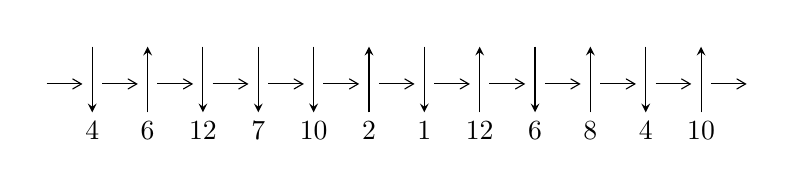
\begin{tikzpicture}[x=20pt, y=17pt]
	% nodes
	\node (C0) at (0, 0) {};
	\node (C1) at (1, 0) {};
	\node (C1U) at (1, +1) {};
	\node (C1D) at (1, -1) {4};

	\node (C2) at (2, 0) {};
	\node (C2U) at (2, +1) {};
	\node (C2D) at (2, -1) {6};

	\node (C3) at (3, 0) {};
	\node (C3U) at (3, +1) {};
	\node (C3D) at (3, -1) {12};

	\node (C4) at (4, 0) {};
	\node (C4U) at (4, +1) {};
	\node (C4D) at (4, -1) {7};

	\node (C5) at (5, 0) {};
	\node (C5U) at (5, +1) {};
	\node (C5D) at (5, -1) {10};

	\node (C6) at (6, 0) {};
	\node (C6U) at (6, +1) {};
	\node (C6D) at (6, -1) {2};

	\node (C7) at (7, 0) {};
	\node (C7U) at (7, +1) {};
	\node (C7D) at (7, -1) {1};

	\node (C8) at (8, 0) {};
	\node (C8U) at (8, +1) {};
	\node (C8D) at (8, -1) {12};

	\node (C9) at (9, 0) {};
	\node (C9U) at (9, +1) {};
	\node (C9D) at (9, -1) {6};

	\node (C10) at (10, 0) {};
	\node (C10U) at (10, +1) {};
	\node (C10D) at (10, -1) {8};

	\node (C11) at (11, 0) {};
	\node (C11U) at (11, +1) {};
	\node (C11D) at (11, -1) {4};

	\node (C12) at (12, 0) {};
	\node (C12U) at (12, +1) {};
	\node (C12D) at (12, -1) {10};
	\node (C13) at (13, 0) {};

	% arrows
	\draw[->,>={angle 60}]
	(C0) edge (C1) (C1) edge (C2) (C2) edge (C3) (C3) edge (C4) (C4) edge (C5) (C5) edge (C6) (C6) edge (C7) (C7) edge (C8) (C8) edge (C9) (C9) edge (C10) (C10) edge (C11) (C11) edge (C12) (C12) edge (C13) ;	\draw[->,>=stealth]
	(C1U) edge (C1D) (C2D) edge (C2U) (C3U) edge (C3D) (C4U) edge (C4D) (C5U) edge (C5D) (C6D) edge (C6U) (C7U) edge (C7D) (C8D) edge (C8U) (C9U) edge (C9D) (C10D) edge (C10U) (C11U) edge (C11D) (C12D) edge (C12U) ;
	\end{tikzpicture} \\
\hhline{~~} \\& 
\textbf{Solving Sequence} \\ \cline{2-2} 
 &
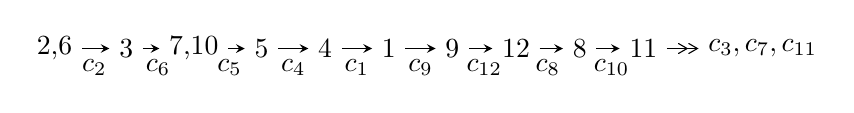
\begin{tikzpicture}[x=23pt, y=7pt]
	% node
	\node (A0) at (-1/8, 0) {2,6};
	\node (A1) at (1, 0) {3};
	\node (A2) at (33/16, 0) {7,10};
	\node (A3) at (25/8, 0) {5};
	\node (A4) at (33/8, 0) {4};
	\node (A5) at (41/8, 0) {1};
	\node (A6) at (49/8, 0) {9};
	\node (A7) at (57/8, 0) {12};
	\node (A8) at (65/8, 0) {8};
	\node (A9) at (73/8, 0) {11};
	\node (C1) at (1/2, -1) {$c_{2}$};
	\node (C2) at (3/2, -1) {$c_{6}$};
	\node (C3) at (21/8, -1) {$c_{5}$};
	\node (C4) at (29/8, -1) {$c_{4}$};
	\node (C5) at (37/8, -1) {$c_{1}$};
	\node (C6) at (45/8, -1) {$c_{9}$};
	\node (C7) at (53/8, -1) {$c_{12}$};
	\node (C8) at (61/8, -1) {$c_{8}$};
	\node (C9) at (69/8, -1) {$c_{10}$};
	\node (A10) at (11, 0) {$c_{3},c_{7},c_{11}$};

	% edge
	\draw[->,>=stealth]	
	(A0) edge (A1) (A1) edge (A2) (A2) edge (A3) (A3) edge (A4) (A4) edge (A5) (A5) edge (A6) (A6) edge (A7) (A7) edge (A8) (A8) edge (A9) ;
	\draw[->>,>={angle 60}]	
	(A9) edge (A10);
\end{tikzpicture} \\ 

\end{tabular} \\

\footnotetext{
The image of knot diagram is generated by the software ``\textbf{Draw programme}" developed by Andrew Bartholomew(\url{http://www.layer8.co.uk/maths/draw/index.htm\#Running-draw}), where we modified some parts for our purpose(\url{https://github.com/CATsTAILs/LinksPainter}).
}\phantom \\ \newline 
\centering \textbf{Ideals for irreducible components\footnotemark of $X_{\text{par}}$} 
 
\begin{align*}
I^u_{1}&=\langle 
5655077 u^{11}+18192667 u^{10}+\cdots+57645040 b+32704792,\\
\phantom{I^u_{1}}&\phantom{= \langle  }4782676 u^{11}+14870711 u^{10}+\cdots+28822520 a+7681096,\\
\phantom{I^u_{1}}&\phantom{= \langle  }u^{12}+4 u^{11}+22 u^{10}+49 u^9+124 u^8+152 u^7+187 u^6+152 u^5+154 u^4+123 u^3+84 u^2+36 u+8\rangle \\
I^u_{2}&=\langle 
- u^8+u^6 a+u^5 a-2 u^6+2 u^4 a-3 u^5+4 u^3 a- u^4+3 u^2 a-3 u^3+3 a u-2 u^2+b+a,\\
\phantom{I^u_{2}}&\phantom{= \langle  }- u^9 a-2 u^8 a+\cdots-2 a-2,\;u^{10}+u^9+3 u^8+6 u^7+7 u^6+9 u^5+10 u^4+8 u^3+5 u^2+2 u+1\rangle \\
I^u_{3}&=\langle 
-5028 u^7 a-3060 u^7+\cdots+87875 a+61205,\\
\phantom{I^u_{3}}&\phantom{= \langle  }-60170 u^7 a-58983 u^7+\cdots+1299250 a+839905,\\
\phantom{I^u_{3}}&\phantom{= \langle  }u^8-6 u^7+24 u^6-50 u^5+73 u^4-72 u^3+61 u^2-55 u+25\rangle \\
I^u_{4}&=\langle 
b- u-1,\;a,\;u^2+u+1\rangle \\
I^u_{5}&=\langle 
u^2+4 b+2 u+5,\;-2 u^2+2 a+3 u-15,\;u^3- u^2+7 u+1\rangle \\
\\
\end{align*}
\raggedright * 5 irreducible components of $\dim_{\mathbb{C}}=0$, with total 53 representations.\\
\footnotetext{All coefficients of polynomials are rational numbers. But the coefficients are sometimes approximated in decimal forms when there is not enough margin.}
\newpage
\renewcommand{\arraystretch}{1}
\centering \section*{I. $I^u_{1}= \langle 5.66\times10^{6} u^{11}+1.82\times10^{7} u^{10}+\cdots+5.76\times10^{7} b+3.27\times10^{7},\;4.78\times10^{6} u^{11}+1.49\times10^{7} u^{10}+\cdots+2.88\times10^{7} a+7.68\times10^{6},\;u^{12}+4 u^{11}+\cdots+36 u+8 \rangle$}
\flushleft \textbf{(i) Arc colorings}\\
\begin{tabular}{m{7pt} m{180pt} m{7pt} m{180pt} }
\flushright $a_{2}=$&$\begin{pmatrix}1\\0\end{pmatrix}$ \\
\flushright $a_{6}=$&$\begin{pmatrix}0\\u\end{pmatrix}$ \\
\flushright $a_{3}=$&$\begin{pmatrix}1\\- u^2\end{pmatrix}$ \\
\flushright $a_{7}=$&$\begin{pmatrix}u\\u\end{pmatrix}$ \\
\flushright $a_{10}=$&$\begin{pmatrix}-0.165935 u^{11}-0.515941 u^{10}+\cdots-3.42377 u-0.266496\\-0.0981017 u^{11}-0.315598 u^{10}+\cdots-1.84222 u-0.567348\end{pmatrix}$ \\
\flushright $a_{5}=$&$\begin{pmatrix}0.0555299 u^{11}+0.197961 u^{10}+\cdots+1.67411 u+1.16096\\-0.0124138 u^{11}-0.0591623 u^{10}+\cdots-0.874760 u-0.426335\end{pmatrix}$ \\
\flushright $a_{4}=$&$\begin{pmatrix}0.0532919 u^{11}+0.200754 u^{10}+\cdots+1.69020 u+1.04375\\-0.0146517 u^{11}-0.0563689 u^{10}+\cdots-0.858673 u-0.543549\end{pmatrix}$ \\
\flushright $a_{1}=$&$\begin{pmatrix}0.0196973 u^{11}+0.0508957 u^{10}+\cdots+1.95987 u+1.74708\\-0.0164741 u^{11}-0.0773159 u^{10}+\cdots-0.265718 u-0.289371\end{pmatrix}$ \\
\flushright $a_{9}=$&$\begin{pmatrix}-0.165935 u^{11}-0.515941 u^{10}+\cdots-3.42377 u-0.266496\\-0.0311444 u^{11}-0.0537009 u^{10}+\cdots+2.15113 u+0.615059\end{pmatrix}$ \\
\flushright $a_{12}=$&$\begin{pmatrix}0.0709185 u^{11}+0.185572 u^{10}+\cdots+1.74180 u+0.710849\\0.0709921 u^{11}+0.228068 u^{10}+\cdots+2.74286 u+0.542669\end{pmatrix}$ \\
\flushright $a_{8}=$&$\begin{pmatrix}-0.0711186 u^{11}-0.224055 u^{10}+\cdots+0.618483 u+0.662628\\0.00749790 u^{11}+0.0714935 u^{10}+\cdots+4.03579 u+0.760724\end{pmatrix}$ \\
\flushright $a_{11}=$&$\begin{pmatrix}-0.164351 u^{11}-0.516002 u^{10}+\cdots-6.02898 u-1.47273\\-0.0364474 u^{11}-0.0811342 u^{10}+\cdots+0.0786132 u+0.481147\end{pmatrix}$\\&\end{tabular}
\flushleft \textbf{(ii) Obstruction class $= -1$}\\~\\
\flushleft \textbf{(iii) Cusp Shapes $= -\frac{728881}{5764504} u^{11}+\frac{352229}{5764504} u^{10}+\cdots+\frac{29077369}{1441126} u+\frac{7367045}{720563}$}\\~\\
\newpage\renewcommand{\arraystretch}{1}
\flushleft \textbf{(iv) u-Polynomials at the component}\newline \\
\begin{tabular}{m{50pt}|m{274pt}}
Crossings & \hspace{64pt}u-Polynomials at each crossing \\
\hline $$\begin{aligned}c_{1},c_{4}\end{aligned}$$&$\begin{aligned}
&u^{12}-4 u^{10}+3 u^9+13 u^8-2 u^7-19 u^6+13 u^4-3 u^3-2 u+1
\end{aligned}$\\
\hline $$\begin{aligned}c_{2},c_{6}\end{aligned}$$&$\begin{aligned}
&u^{12}-4 u^{11}+\cdots-36 u+8
\end{aligned}$\\
\hline $$\begin{aligned}c_{3},c_{5},c_{9}\\c_{11}\end{aligned}$$&$\begin{aligned}
&u^{12}+5 u^{11}+\cdots+16 u+4
\end{aligned}$\\
\hline $$\begin{aligned}c_{7}\end{aligned}$$&$\begin{aligned}
&u^{12}-12 u^{11}+\cdots-112 u+16
\end{aligned}$\\
\hline $$\begin{aligned}c_{8}\end{aligned}$$&$\begin{aligned}
&u^{12}-13 u^{11}+\cdots-2840 u+472
\end{aligned}$\\
\hline $$\begin{aligned}c_{10},c_{12}\end{aligned}$$&$\begin{aligned}
&u^{12}- u^{11}+\cdots- u+1
\end{aligned}$\\
\hline
\end{tabular}\\~\\
\newpage\renewcommand{\arraystretch}{1}
\flushleft \textbf{(v) Riley Polynomials at the component}\newline \\
\begin{tabular}{m{50pt}|m{274pt}}
Crossings & \hspace{64pt}Riley Polynomials at each crossing \\
\hline $$\begin{aligned}c_{1},c_{4}\end{aligned}$$&$\begin{aligned}
&y^{12}-8 y^{11}+\cdots-4 y+1
\end{aligned}$\\
\hline $$\begin{aligned}c_{2},c_{6}\end{aligned}$$&$\begin{aligned}
&y^{12}+28 y^{11}+\cdots+48 y+64
\end{aligned}$\\
\hline $$\begin{aligned}c_{3},c_{5},c_{9}\\c_{11}\end{aligned}$$&$\begin{aligned}
&y^{12}-23 y^{11}+\cdots+192 y+16
\end{aligned}$\\
\hline $$\begin{aligned}c_{7}\end{aligned}$$&$\begin{aligned}
&y^{12}+2 y^{11}+\cdots+1536 y+256
\end{aligned}$\\
\hline $$\begin{aligned}c_{8}\end{aligned}$$&$\begin{aligned}
&y^{12}+45 y^{11}+\cdots+1504672 y+222784
\end{aligned}$\\
\hline $$\begin{aligned}c_{10},c_{12}\end{aligned}$$&$\begin{aligned}
&y^{12}- y^{11}+\cdots+31 y+1
\end{aligned}$\\
\hline
\end{tabular}\\~\\
\newpage\flushleft \textbf{(vi) Complex Volumes and Cusp Shapes}
$$\begin{array}{c|c|c}  
\text{Solutions to }I^u_{1}& \I (\text{vol} + \sqrt{-1}CS) & \text{Cusp shape}\\
 \hline 
\begin{aligned}
u &= \phantom{-}0.540143 + 0.761627 I \\
a &= -1.69223 + 0.78856 I \\
b &= -0.993599 + 0.115131 I\end{aligned}
 & -2.97909 + 0.17410 I & -3.65502 - 0.56316 I \\ \hline\begin{aligned}
u &= \phantom{-}0.540143 - 0.761627 I \\
a &= -1.69223 - 0.78856 I \\
b &= -0.993599 - 0.115131 I\end{aligned}
 & -2.97909 - 0.17410 I & -3.65502 + 0.56316 I \\ \hline\begin{aligned}
u &= -0.495932 + 0.959152 I \\
a &= \phantom{-}0.436587 - 0.071368 I \\
b &= \phantom{-}0.788354 - 0.737396 I\end{aligned}
 & -0.33260 - 5.31098 I & \phantom{-}0.92797 + 6.12254 I \\ \hline\begin{aligned}
u &= -0.495932 - 0.959152 I \\
a &= \phantom{-}0.436587 + 0.071368 I \\
b &= \phantom{-}0.788354 + 0.737396 I\end{aligned}
 & -0.33260 + 5.31098 I & \phantom{-}0.92797 - 6.12254 I \\ \hline\begin{aligned}
u &= -0.313071 + 0.674527 I \\
a &= -0.261436 + 0.583661 I \\
b &= \phantom{-}0.024504 + 0.511749 I\end{aligned}
 & -0.252110 - 1.156370 I & -2.57186 + 6.15407 I \\ \hline\begin{aligned}
u &= -0.313071 - 0.674527 I \\
a &= -0.261436 - 0.583661 I \\
b &= \phantom{-}0.024504 - 0.511749 I\end{aligned}
 & -0.252110 + 1.156370 I & -2.57186 - 6.15407 I \\ \hline\begin{aligned}
u &= -0.433831 + 0.256446 I \\
a &= \phantom{-}0.396072 - 1.201640 I \\
b &= -0.339334 - 0.183220 I\end{aligned}
 & \phantom{-}1.23387 + 1.55175 I & \phantom{-}4.02015 - 1.83829 I \\ \hline\begin{aligned}
u &= -0.433831 - 0.256446 I \\
a &= \phantom{-}0.396072 + 1.201640 I \\
b &= -0.339334 + 0.183220 I\end{aligned}
 & \phantom{-}1.23387 - 1.55175 I & \phantom{-}4.02015 + 1.83829 I \\ \hline\begin{aligned}
u &= -0.29653 + 2.66870 I \\
a &= -0.147885 - 0.838892 I \\
b &= \phantom{-}0.05531 - 2.12763 I\end{aligned}
 & -16.8158 - 1.6628 I & -7.43215 + 4.58115 I \\ \hline\begin{aligned}
u &= -0.29653 - 2.66870 I \\
a &= -0.147885 + 0.838892 I \\
b &= \phantom{-}0.05531 + 2.12763 I\end{aligned}
 & -16.8158 + 1.6628 I & -7.43215 - 4.58115 I\\
 \hline 
 \end{array}$$\newpage$$\begin{array}{c|c|c}  
\text{Solutions to }I^u_{1}& \I (\text{vol} + \sqrt{-1}CS) & \text{Cusp shape}\\
 \hline 
\begin{aligned}
u &= -1.00078 + 2.60205 I \\
a &= -0.231108 + 1.220450 I \\
b &= -0.03524 + 2.20216 I\end{aligned}
 & \phantom{-}18.3232 - 12.8945 I & -2.78911 + 4.52447 I \\ \hline\begin{aligned}
u &= -1.00078 - 2.60205 I \\
a &= -0.231108 - 1.220450 I \\
b &= -0.03524 - 2.20216 I\end{aligned}
 & \phantom{-}18.3232 + 12.8945 I & -2.78911 - 4.52447 I\\
 \hline 
 \end{array}$$\newpage\newpage\renewcommand{\arraystretch}{1}
\centering \section*{II. $I^u_{2}= \langle - u^8+u^6 a+\cdots+b+a,\;- u^9 a-2 u^8 a+\cdots-2 a-2,\;u^{10}+u^9+\cdots+2 u+1 \rangle$}
\flushleft \textbf{(i) Arc colorings}\\
\begin{tabular}{m{7pt} m{180pt} m{7pt} m{180pt} }
\flushright $a_{2}=$&$\begin{pmatrix}1\\0\end{pmatrix}$ \\
\flushright $a_{6}=$&$\begin{pmatrix}0\\u\end{pmatrix}$ \\
\flushright $a_{3}=$&$\begin{pmatrix}1\\- u^2\end{pmatrix}$ \\
\flushright $a_{7}=$&$\begin{pmatrix}u\\u\end{pmatrix}$ \\
\flushright $a_{10}=$&$\begin{pmatrix}a\\u^8- u^6 a+\cdots-3 a u- a\end{pmatrix}$ \\
\flushright $a_{5}=$&$\begin{pmatrix}u^9 a+u^9+\cdots- a+2 u\\u^9 a+u^9+\cdots+a+2\end{pmatrix}$ \\
\flushright $a_{4}=$&$\begin{pmatrix}u^9 a+u^9+\cdots-2 a+2 u\\u^9 a+u^9+\cdots+5 u+2\end{pmatrix}$ \\
\flushright $a_{1}=$&$\begin{pmatrix}- u^9 a- u^9+\cdots-6 u-1\\- u^9 a- u^9+\cdots-4 u-1\end{pmatrix}$ \\
\flushright $a_{9}=$&$\begin{pmatrix}a\\u^8- u^6 a+\cdots-3 a u- a\end{pmatrix}$ \\
\flushright $a_{12}=$&$\begin{pmatrix}- u^9 a-2 u^9+\cdots+a-2\\- u^7 a- u^8+\cdots-4 u-2\end{pmatrix}$ \\
\flushright $a_{8}=$&$\begin{pmatrix}u^8 a+3 u^9+\cdots- a u+6 u\\u^8 a+u^9+\cdots+6 u+2\end{pmatrix}$ \\
\flushright $a_{11}=$&$\begin{pmatrix}- u^9 a-2 u^9+\cdots+2 a-1\\- u^7 a-2 u^8+\cdots+a-3\end{pmatrix}$\\&\end{tabular}
\flushleft \textbf{(ii) Obstruction class $= 1$}\\~\\
\flushleft \textbf{(iii) Cusp Shapes $= 2 u^9+u^8+9 u^7+17 u^6+17 u^5+31 u^4+34 u^3+19 u^2+15 u+2$}\\~\\
\newpage\renewcommand{\arraystretch}{1}
\flushleft \textbf{(iv) u-Polynomials at the component}\newline \\
\begin{tabular}{m{50pt}|m{274pt}}
Crossings & \hspace{64pt}u-Polynomials at each crossing \\
\hline $$\begin{aligned}c_{1},c_{4}\end{aligned}$$&$\begin{aligned}
&u^{20}-7 u^{19}+\cdots-7 u+1
\end{aligned}$\\
\hline $$\begin{aligned}c_{2}\end{aligned}$$&$\begin{aligned}
&(u^{10}+u^9+3 u^8+6 u^7+7 u^6+9 u^5+10 u^4+8 u^3+5 u^2+2 u+1)^2
\end{aligned}$\\
\hline $$\begin{aligned}c_{3},c_{9}\end{aligned}$$&$\begin{aligned}
&u^{20}+4 u^{19}+\cdots+24 u+4
\end{aligned}$\\
\hline $$\begin{aligned}c_{5},c_{11}\end{aligned}$$&$\begin{aligned}
&u^{20}-4 u^{19}+\cdots-24 u+4
\end{aligned}$\\
\hline $$\begin{aligned}c_{6}\end{aligned}$$&$\begin{aligned}
&(u^{10}- u^9+3 u^8-6 u^7+7 u^6-9 u^5+10 u^4-8 u^3+5 u^2-2 u+1)^2
\end{aligned}$\\
\hline $$\begin{aligned}c_{7}\end{aligned}$$&$\begin{aligned}
&(u^{10}-4 u^8+10 u^6-2 u^5-9 u^4-12 u^3+15 u^2+2 u+4)^2
\end{aligned}$\\
\hline $$\begin{aligned}c_{8}\end{aligned}$$&$\begin{aligned}
&(u^{10}+2 u^9-4 u^8-4 u^7+14 u^6+6 u^5-14 u^4-4 u^3+12 u^2+6 u+1)^2
\end{aligned}$\\
\hline $$\begin{aligned}c_{10},c_{12}\end{aligned}$$&$\begin{aligned}
&u^{20}-7 u^{19}+\cdots-6 u+1
\end{aligned}$\\
\hline
\end{tabular}\\~\\
\newpage\renewcommand{\arraystretch}{1}
\flushleft \textbf{(v) Riley Polynomials at the component}\newline \\
\begin{tabular}{m{50pt}|m{274pt}}
Crossings & \hspace{64pt}Riley Polynomials at each crossing \\
\hline $$\begin{aligned}c_{1},c_{4}\end{aligned}$$&$\begin{aligned}
&y^{20}- y^{19}+\cdots-9 y+1
\end{aligned}$\\
\hline $$\begin{aligned}c_{2},c_{6}\end{aligned}$$&$\begin{aligned}
&(y^{10}+5 y^9+11 y^8+8 y^7-5 y^6-9 y^5+8 y^4+14 y^3+13 y^2+6 y+1)^2
\end{aligned}$\\
\hline $$\begin{aligned}c_{3},c_{5},c_{9}\\c_{11}\end{aligned}$$&$\begin{aligned}
&y^{20}+2 y^{19}+\cdots+64 y+16
\end{aligned}$\\
\hline $$\begin{aligned}c_{7}\end{aligned}$$&$\begin{aligned}
&(y^{10}-8 y^9+\cdots+116 y+16)^{2}
\end{aligned}$\\
\hline $$\begin{aligned}c_{8}\end{aligned}$$&$\begin{aligned}
&(y^{10}-12 y^9+\cdots-12 y+1)^{2}
\end{aligned}$\\
\hline $$\begin{aligned}c_{10},c_{12}\end{aligned}$$&$\begin{aligned}
&y^{20}-9 y^{19}+\cdots-8 y+1
\end{aligned}$\\
\hline
\end{tabular}\\~\\
\newpage\flushleft \textbf{(vi) Complex Volumes and Cusp Shapes}
$$\begin{array}{c|c|c}  
\text{Solutions to }I^u_{2}& \I (\text{vol} + \sqrt{-1}CS) & \text{Cusp shape}\\
 \hline 
\begin{aligned}
u &= -1.014310 + 0.256691 I \\
a &= \phantom{-}0.964180 - 0.567184 I \\
b &= -0.172201 - 1.125270 I\end{aligned}
 & -2.82507 - 0.01586 I & -5.03096 + 0.40672 I \\ \hline\begin{aligned}
u &= -1.014310 + 0.256691 I \\
a &= \phantom{-}0.842936 + 0.896392 I \\
b &= -0.089370 + 1.110650 I\end{aligned}
 & -2.82507 - 0.01586 I & -5.03096 + 0.40672 I \\ \hline\begin{aligned}
u &= -1.014310 - 0.256691 I \\
a &= \phantom{-}0.964180 + 0.567184 I \\
b &= -0.172201 + 1.125270 I\end{aligned}
 & -2.82507 + 0.01586 I & -5.03096 - 0.40672 I \\ \hline\begin{aligned}
u &= -1.014310 - 0.256691 I \\
a &= \phantom{-}0.842936 - 0.896392 I \\
b &= -0.089370 - 1.110650 I\end{aligned}
 & -2.82507 + 0.01586 I & -5.03096 - 0.40672 I \\ \hline\begin{aligned}
u &= -0.494190 + 0.650032 I \\
a &= \phantom{-}0.701854 - 0.119057 I \\
b &= \phantom{-}0.93649 - 2.03449 I\end{aligned}
 & -1.80674 - 6.46947 I & -1.01128 + 9.30231 I \\ \hline\begin{aligned}
u &= -0.494190 + 0.650032 I \\
a &= -0.366624 - 1.277610 I \\
b &= \phantom{-}0.159063 - 0.249786 I\end{aligned}
 & -1.80674 - 6.46947 I & -1.01128 + 9.30231 I \\ \hline\begin{aligned}
u &= -0.494190 - 0.650032 I \\
a &= \phantom{-}0.701854 + 0.119057 I \\
b &= \phantom{-}0.93649 + 2.03449 I\end{aligned}
 & -1.80674 + 6.46947 I & -1.01128 - 9.30231 I \\ \hline\begin{aligned}
u &= -0.494190 - 0.650032 I \\
a &= -0.366624 + 1.277610 I \\
b &= \phantom{-}0.159063 + 0.249786 I\end{aligned}
 & -1.80674 + 6.46947 I & -1.01128 - 9.30231 I \\ \hline\begin{aligned}
u &= \phantom{-}0.382212 + 1.255980 I \\
a &= \phantom{-}0.293033 - 1.100270 I \\
b &= \phantom{-}0.11581 - 2.62267 I\end{aligned}
 & -3.73684 + 4.80030 I & -9.38054 - 3.15587 I \\ \hline\begin{aligned}
u &= \phantom{-}0.382212 + 1.255980 I \\
a &= -0.519971 + 0.035643 I \\
b &= -0.588255 + 0.303305 I\end{aligned}
 & -3.73684 + 4.80030 I & -9.38054 - 3.15587 I\\
 \hline 
 \end{array}$$\newpage$$\begin{array}{c|c|c}  
\text{Solutions to }I^u_{2}& \I (\text{vol} + \sqrt{-1}CS) & \text{Cusp shape}\\
 \hline 
\begin{aligned}
u &= \phantom{-}0.382212 - 1.255980 I \\
a &= \phantom{-}0.293033 + 1.100270 I \\
b &= \phantom{-}0.11581 + 2.62267 I\end{aligned}
 & -3.73684 - 4.80030 I & -9.38054 + 3.15587 I \\ \hline\begin{aligned}
u &= \phantom{-}0.382212 - 1.255980 I \\
a &= -0.519971 - 0.035643 I \\
b &= -0.588255 - 0.303305 I\end{aligned}
 & -3.73684 - 4.80030 I & -9.38054 + 3.15587 I \\ \hline\begin{aligned}
u &= \phantom{-}0.068366 + 0.610240 I \\
a &= -0.187485 + 1.399550 I \\
b &= \phantom{-}0.909534 - 0.136013 I\end{aligned}
 & -0.72327 - 2.84641 I & -2.67521 + 3.01300 I \\ \hline\begin{aligned}
u &= \phantom{-}0.068366 + 0.610240 I \\
a &= -1.41876 + 0.52381 I \\
b &= -0.061464 + 1.381430 I\end{aligned}
 & -0.72327 - 2.84641 I & -2.67521 + 3.01300 I \\ \hline\begin{aligned}
u &= \phantom{-}0.068366 - 0.610240 I \\
a &= -0.187485 - 1.399550 I \\
b &= \phantom{-}0.909534 + 0.136013 I\end{aligned}
 & -0.72327 + 2.84641 I & -2.67521 - 3.01300 I \\ \hline\begin{aligned}
u &= \phantom{-}0.068366 - 0.610240 I \\
a &= -1.41876 - 0.52381 I \\
b &= -0.061464 - 1.381430 I\end{aligned}
 & -0.72327 + 2.84641 I & -2.67521 - 3.01300 I \\ \hline\begin{aligned}
u &= \phantom{-}0.55792 + 1.34043 I \\
a &= \phantom{-}0.830798 + 0.641959 I \\
b &= -0.21457 + 2.05660 I\end{aligned}
 & \phantom{-}5.80206 + 1.85988 I & \phantom{-}11.59799 + 1.32723 I \\ \hline\begin{aligned}
u &= \phantom{-}0.55792 + 1.34043 I \\
a &= -1.139960 - 0.180068 I \\
b &= -0.495038 - 0.305606 I\end{aligned}
 & \phantom{-}5.80206 + 1.85988 I & \phantom{-}11.59799 + 1.32723 I \\ \hline\begin{aligned}
u &= \phantom{-}0.55792 - 1.34043 I \\
a &= \phantom{-}0.830798 - 0.641959 I \\
b &= -0.21457 - 2.05660 I\end{aligned}
 & \phantom{-}5.80206 - 1.85988 I & \phantom{-}11.59799 - 1.32723 I \\ \hline\begin{aligned}
u &= \phantom{-}0.55792 - 1.34043 I \\
a &= -1.139960 + 0.180068 I \\
b &= -0.495038 + 0.305606 I\end{aligned}
 & \phantom{-}5.80206 - 1.85988 I & \phantom{-}11.59799 - 1.32723 I\\
 \hline 
 \end{array}$$\newpage\newpage\renewcommand{\arraystretch}{1}
\centering \section*{III. $I^u_{3}= \langle -5028 u^7 a-3060 u^7+\cdots+87875 a+61205,\;-6.02\times10^{4} a u^{7}-5.90\times10^{4} u^{7}+\cdots+1.30\times10^{6} a+8.40\times10^{5},\;u^8-6 u^7+\cdots-55 u+25 \rangle$}
\flushleft \textbf{(i) Arc colorings}\\
\begin{tabular}{m{7pt} m{180pt} m{7pt} m{180pt} }
\flushright $a_{2}=$&$\begin{pmatrix}1\\0\end{pmatrix}$ \\
\flushright $a_{6}=$&$\begin{pmatrix}0\\u\end{pmatrix}$ \\
\flushright $a_{3}=$&$\begin{pmatrix}1\\- u^2\end{pmatrix}$ \\
\flushright $a_{7}=$&$\begin{pmatrix}u\\u\end{pmatrix}$ \\
\flushright $a_{10}=$&$\begin{pmatrix}a\\0.208156 a u^{7}+0.126682 u^{7}+\cdots-3.63796 a-2.53384\end{pmatrix}$ \\
\flushright $a_{5}=$&$\begin{pmatrix}0.0470296 a u^{7}+0.0807038 u^{7}+\cdots-2.49100 a-2.44185\\-0.0371352 a u^{7}+0.0705030 u^{7}+\cdots+0.0672739 a-0.0987373\end{pmatrix}$ \\
\flushright $a_{4}=$&$\begin{pmatrix}0.00269095 a u^{7}+0.0452660 u^{7}+\cdots-0.454150 a-2.52258\\-0.0814738 a u^{7}+0.0350652 u^{7}+\cdots+2.10412 a-0.179466\end{pmatrix}$ \\
\flushright $a_{1}=$&$\begin{pmatrix}-0.0475678 a u^{7}-0.0396357 u^{7}+\cdots-1.21817 a+2.58775\\-0.0475678 a u^{7}-0.0895467 u^{7}+\cdots-1.21817 a+2.46657\end{pmatrix}$ \\
\flushright $a_{9}=$&$\begin{pmatrix}a\\0.208156 a u^{7}+0.126682 u^{7}+\cdots-3.63796 a-2.53384\end{pmatrix}$ \\
\flushright $a_{12}=$&$\begin{pmatrix}-0.145519 a u^{7}-0.0181660 u^{7}+\cdots+2.71290 a+0.0474022\\0.192548 a u^{7}+0.0841648 u^{7}+\cdots-5.20389 a-2.55827\end{pmatrix}$ \\
\flushright $a_{8}=$&$\begin{pmatrix}0.128379 a u^{7}+0.0664376 u^{7}+\cdots-1.68185 a-0.471083\\0.128379 a u^{7}+0.313310 u^{7}+\cdots-1.68185 a-5.53860\end{pmatrix}$ \\
\flushright $a_{11}=$&$\begin{pmatrix}0.106189 a u^{7}+0.234602 u^{7}+\cdots-3.84455 a-1.23660\\-0.228648 a u^{7}+0.0835438 u^{7}+\cdots+4.32726 a+2.00807\end{pmatrix}$\\&\end{tabular}
\flushleft \textbf{(ii) Obstruction class $= -1$}\\~\\
\flushleft \textbf{(iii) Cusp Shapes $= \frac{2475}{4831} u^7-\frac{58067}{24155} u^6+\frac{218393}{24155} u^5-\frac{326712}{24155} u^4+\frac{446026}{24155} u^3-\frac{285694}{24155} u^2+\frac{252936}{24155} u-\frac{68757}{4831}$}\\~\\
\newpage\renewcommand{\arraystretch}{1}
\flushleft \textbf{(iv) u-Polynomials at the component}\newline \\
\begin{tabular}{m{50pt}|m{274pt}}
Crossings & \hspace{64pt}u-Polynomials at each crossing \\
\hline $$\begin{aligned}c_{1},c_{4}\end{aligned}$$&$\begin{aligned}
&u^{16}-5 u^{15}+\cdots-137 u+103
\end{aligned}$\\
\hline $$\begin{aligned}c_{2},c_{6}\end{aligned}$$&$\begin{aligned}
&(u^8+6 u^7+24 u^6+50 u^5+73 u^4+72 u^3+61 u^2+55 u+25)^2
\end{aligned}$\\
\hline $$\begin{aligned}c_{3},c_{5},c_{9}\\c_{11}\end{aligned}$$&$\begin{aligned}
&u^{16}-4 u^{15}+\cdots+8104 u+8557
\end{aligned}$\\
\hline $$\begin{aligned}c_{7}\end{aligned}$$&$\begin{aligned}
&(u^4+2 u^3-3 u-1)^4
\end{aligned}$\\
\hline $$\begin{aligned}c_{8}\end{aligned}$$&$\begin{aligned}
&(u^8+4 u^7+\cdots+1636 u+709)^{2}
\end{aligned}$\\
\hline $$\begin{aligned}c_{10},c_{12}\end{aligned}$$&$\begin{aligned}
&u^{16}+5 u^{15}+\cdots+1490 u+631
\end{aligned}$\\
\hline
\end{tabular}\\~\\
\newpage\renewcommand{\arraystretch}{1}
\flushleft \textbf{(v) Riley Polynomials at the component}\newline \\
\begin{tabular}{m{50pt}|m{274pt}}
Crossings & \hspace{64pt}Riley Polynomials at each crossing \\
\hline $$\begin{aligned}c_{1},c_{4}\end{aligned}$$&$\begin{aligned}
&y^{16}-3 y^{15}+\cdots-68415 y+10609
\end{aligned}$\\
\hline $$\begin{aligned}c_{2},c_{6}\end{aligned}$$&$\begin{aligned}
&(y^8+12 y^7+122 y^6+262 y^5+447 y^4-578 y^3-549 y^2+25 y+625)^{2}
\end{aligned}$\\
\hline $$\begin{aligned}c_{3},c_{5},c_{9}\\c_{11}\end{aligned}$$&$\begin{aligned}
&y^{16}-42 y^{15}+\cdots+743954296 y+73222249
\end{aligned}$\\
\hline $$\begin{aligned}c_{7}\end{aligned}$$&$\begin{aligned}
&(y^4-4 y^3+10 y^2-9 y+1)^4
\end{aligned}$\\
\hline $$\begin{aligned}c_{8}\end{aligned}$$&$\begin{aligned}
&(y^8+110 y^7+\cdots+929478 y+502681)^{2}
\end{aligned}$\\
\hline $$\begin{aligned}c_{10},c_{12}\end{aligned}$$&$\begin{aligned}
&y^{16}-17 y^{15}+\cdots+2691604 y+398161
\end{aligned}$\\
\hline
\end{tabular}\\~\\
\newpage\flushleft \textbf{(vi) Complex Volumes and Cusp Shapes}
$$\begin{array}{c|c|c}  
\text{Solutions to }I^u_{3}& \I (\text{vol} + \sqrt{-1}CS) & \text{Cusp shape}\\
 \hline 
\begin{aligned}
u &= -0.356173 + 0.922051 I \\
a &= -1.45726 - 0.66205 I \\
b &= -0.571202 + 0.124651 I\end{aligned}
 & -2.60769 + 5.61159 I & -4.01448 - 3.52119 I \\ \hline\begin{aligned}
u &= -0.356173 + 0.922051 I \\
a &= \phantom{-}0.58952 - 1.50850 I \\
b &= -0.46449 - 2.42477 I\end{aligned}
 & -2.60769 + 5.61159 I & -4.01448 - 3.52119 I \\ \hline\begin{aligned}
u &= -0.356173 - 0.922051 I \\
a &= -1.45726 + 0.66205 I \\
b &= -0.571202 - 0.124651 I\end{aligned}
 & -2.60769 - 5.61159 I & -4.01448 + 3.52119 I \\ \hline\begin{aligned}
u &= -0.356173 - 0.922051 I \\
a &= \phantom{-}0.58952 + 1.50850 I \\
b &= -0.46449 + 2.42477 I\end{aligned}
 & -2.60769 - 5.61159 I & -4.01448 + 3.52119 I \\ \hline\begin{aligned}
u &= \phantom{-}0.976606 + 0.152571 I \\
a &= -1.248430 - 0.212849 I \\
b &= \phantom{-}0.444438 - 0.330170 I\end{aligned}
 & -2.60769 - 1.55182 I & -4.60507 + 3.15648 I \\ \hline\begin{aligned}
u &= \phantom{-}0.976606 + 0.152571 I \\
a &= -0.065632 + 0.390479 I \\
b &= \phantom{-}0.386763 + 1.198400 I\end{aligned}
 & -2.60769 - 1.55182 I & -4.60507 + 3.15648 I \\ \hline\begin{aligned}
u &= \phantom{-}0.976606 - 0.152571 I \\
a &= -1.248430 + 0.212849 I \\
b &= \phantom{-}0.444438 + 0.330170 I\end{aligned}
 & -2.60769 + 1.55182 I & -4.60507 - 3.15648 I \\ \hline\begin{aligned}
u &= \phantom{-}0.976606 - 0.152571 I \\
a &= -0.065632 - 0.390479 I \\
b &= \phantom{-}0.386763 - 1.198400 I\end{aligned}
 & -2.60769 + 1.55182 I & -4.60507 - 3.15648 I \\ \hline\begin{aligned}
u &= \phantom{-}0.82072 + 1.42153 I \\
a &= \phantom{-}0.883685 + 0.700209 I \\
b &= -0.16909 + 1.79182 I\end{aligned}
 & \phantom{-}5.45104 + 2.02988 I & -7.20164 - 6.73627 I \\ \hline\begin{aligned}
u &= \phantom{-}0.82072 + 1.42153 I \\
a &= \phantom{-}1.150180 + 0.122308 I \\
b &= \phantom{-}0.512857 + 0.312984 I\end{aligned}
 & \phantom{-}5.45104 + 2.02988 I & -7.20164 - 6.73627 I\\
 \hline 
 \end{array}$$\newpage$$\begin{array}{c|c|c}  
\text{Solutions to }I^u_{3}& \I (\text{vol} + \sqrt{-1}CS) & \text{Cusp shape}\\
 \hline 
\begin{aligned}
u &= \phantom{-}0.82072 - 1.42153 I \\
a &= \phantom{-}0.883685 - 0.700209 I \\
b &= -0.16909 - 1.79182 I\end{aligned}
 & \phantom{-}5.45104 - 2.02988 I & -7.20164 + 6.73627 I \\ \hline\begin{aligned}
u &= \phantom{-}0.82072 - 1.42153 I \\
a &= \phantom{-}1.150180 - 0.122308 I \\
b &= \phantom{-}0.512857 - 0.312984 I\end{aligned}
 & \phantom{-}5.45104 - 2.02988 I & -7.20164 + 6.73627 I \\ \hline\begin{aligned}
u &= \phantom{-}1.55884 + 2.70000 I \\
a &= \phantom{-}0.40664 - 1.37969 I \\
b &= \phantom{-}0.37568 - 2.03120 I\end{aligned}
 & \phantom{-}19.5035 + 2.0299 I & -3.67881 - 0.69325 I \\ \hline\begin{aligned}
u &= \phantom{-}1.55884 + 2.70000 I \\
a &= \phantom{-}0.14130 + 1.51086 I \\
b &= -0.01496 + 2.22431 I\end{aligned}
 & \phantom{-}19.5035 + 2.0299 I & -3.67881 - 0.69325 I \\ \hline\begin{aligned}
u &= \phantom{-}1.55884 - 2.70000 I \\
a &= \phantom{-}0.40664 + 1.37969 I \\
b &= \phantom{-}0.37568 + 2.03120 I\end{aligned}
 & \phantom{-}19.5035 - 2.0299 I & -3.67881 + 0.69325 I \\ \hline\begin{aligned}
u &= \phantom{-}1.55884 - 2.70000 I \\
a &= \phantom{-}0.14130 - 1.51086 I \\
b &= -0.01496 - 2.22431 I\end{aligned}
 & \phantom{-}19.5035 - 2.0299 I & -3.67881 + 0.69325 I\\
 \hline 
 \end{array}$$\newpage\newpage\renewcommand{\arraystretch}{1}
\centering \section*{IV. $I^u_{4}= \langle b- u-1,\;a,\;u^2+u+1 \rangle$}
\flushleft \textbf{(i) Arc colorings}\\
\begin{tabular}{m{7pt} m{180pt} m{7pt} m{180pt} }
\flushright $a_{2}=$&$\begin{pmatrix}1\\0\end{pmatrix}$ \\
\flushright $a_{6}=$&$\begin{pmatrix}0\\u\end{pmatrix}$ \\
\flushright $a_{3}=$&$\begin{pmatrix}1\\u+1\end{pmatrix}$ \\
\flushright $a_{7}=$&$\begin{pmatrix}u\\u\end{pmatrix}$ \\
\flushright $a_{10}=$&$\begin{pmatrix}0\\u+1\end{pmatrix}$ \\
\flushright $a_{5}=$&$\begin{pmatrix}0\\u\end{pmatrix}$ \\
\flushright $a_{4}=$&$\begin{pmatrix}1\\u+1\end{pmatrix}$ \\
\flushright $a_{1}=$&$\begin{pmatrix}- u\\- u\end{pmatrix}$ \\
\flushright $a_{9}=$&$\begin{pmatrix}0\\u+1\end{pmatrix}$ \\
\flushright $a_{12}=$&$\begin{pmatrix}- u\\1\end{pmatrix}$ \\
\flushright $a_{8}=$&$\begin{pmatrix}u\\u\end{pmatrix}$ \\
\flushright $a_{11}=$&$\begin{pmatrix}- u\\1\end{pmatrix}$\\&\end{tabular}
\flushleft \textbf{(ii) Obstruction class $= 1$}\\~\\
\flushleft \textbf{(iii) Cusp Shapes $= 4 u+2$}\\~\\
\newpage\renewcommand{\arraystretch}{1}
\flushleft \textbf{(iv) u-Polynomials at the component}\newline \\
\begin{tabular}{m{50pt}|m{274pt}}
Crossings & \hspace{64pt}u-Polynomials at each crossing \\
\hline $$\begin{aligned}c_{1},c_{4},c_{6}\end{aligned}$$&$\begin{aligned}
&u^2- u+1
\end{aligned}$\\
\hline $$\begin{aligned}c_{2}\end{aligned}$$&$\begin{aligned}
&u^2+u+1
\end{aligned}$\\
\hline $$\begin{aligned}c_{3},c_{5},c_{7}\\c_{9},c_{11}\end{aligned}$$&$\begin{aligned}
&u^2
\end{aligned}$\\
\hline $$\begin{aligned}c_{8}\end{aligned}$$&$\begin{aligned}
&(u+1)^2
\end{aligned}$\\
\hline $$\begin{aligned}c_{10},c_{12}\end{aligned}$$&$\begin{aligned}
&(u-1)^2
\end{aligned}$\\
\hline
\end{tabular}\\~\\
\newpage\renewcommand{\arraystretch}{1}
\flushleft \textbf{(v) Riley Polynomials at the component}\newline \\
\begin{tabular}{m{50pt}|m{274pt}}
Crossings & \hspace{64pt}Riley Polynomials at each crossing \\
\hline $$\begin{aligned}c_{1},c_{2},c_{4}\\c_{6}\end{aligned}$$&$\begin{aligned}
&y^2+y+1
\end{aligned}$\\
\hline $$\begin{aligned}c_{3},c_{5},c_{7}\\c_{9},c_{11}\end{aligned}$$&$\begin{aligned}
&y^2
\end{aligned}$\\
\hline $$\begin{aligned}c_{8},c_{10},c_{12}\end{aligned}$$&$\begin{aligned}
&(y-1)^2
\end{aligned}$\\
\hline
\end{tabular}\\~\\
\newpage\flushleft \textbf{(vi) Complex Volumes and Cusp Shapes}
$$\begin{array}{c|c|c}  
\text{Solutions to }I^u_{4}& \I (\text{vol} + \sqrt{-1}CS) & \text{Cusp shape}\\
 \hline 
\begin{aligned}
u &= -0.500000 + 0.866025 I \\
a &= \phantom{-0.000000 } 0 \\
b &= \phantom{-}0.500000 + 0.866025 I\end{aligned}
 & \phantom{-}1.64493 - 2.02988 I & \phantom{-0.000000 -}0. + 3.46410 I \\ \hline\begin{aligned}
u &= -0.500000 - 0.866025 I \\
a &= \phantom{-0.000000 } 0 \\
b &= \phantom{-}0.500000 - 0.866025 I\end{aligned}
 & \phantom{-}1.64493 + 2.02988 I & \phantom{-0.000000 } 0. - 3.46410 I\\
 \hline 
 \end{array}$$\newpage\newpage\renewcommand{\arraystretch}{1}
\centering \section*{V. $I^u_{5}= \langle u^2+4 b+2 u+5,\;-2 u^2+2 a+3 u-15,\;u^3- u^2+7 u+1 \rangle$}
\flushleft \textbf{(i) Arc colorings}\\
\begin{tabular}{m{7pt} m{180pt} m{7pt} m{180pt} }
\flushright $a_{2}=$&$\begin{pmatrix}1\\0\end{pmatrix}$ \\
\flushright $a_{6}=$&$\begin{pmatrix}0\\u\end{pmatrix}$ \\
\flushright $a_{3}=$&$\begin{pmatrix}1\\- u^2\end{pmatrix}$ \\
\flushright $a_{7}=$&$\begin{pmatrix}u\\u\end{pmatrix}$ \\
\flushright $a_{10}=$&$\begin{pmatrix}u^2-\frac{3}{2} u+\frac{15}{2}\\-\frac{1}{4} u^2-\frac{1}{2} u-\frac{5}{4}\end{pmatrix}$ \\
\flushright $a_{5}=$&$\begin{pmatrix}-\frac{5}{4} u^2+\frac{1}{2} u-\frac{33}{4}\\- u+1\end{pmatrix}$ \\
\flushright $a_{4}=$&$\begin{pmatrix}- u^2+u-8\\\frac{1}{4} u^2-\frac{1}{2} u+\frac{5}{4}\end{pmatrix}$ \\
\flushright $a_{1}=$&$\begin{pmatrix}\frac{3}{2} u^2-2 u+\frac{23}{2}\\-\frac{1}{4} u^2-\frac{7}{4}\end{pmatrix}$ \\
\flushright $a_{9}=$&$\begin{pmatrix}u^2-\frac{3}{2} u+\frac{15}{2}\\-\frac{1}{4} u^2-3 u-\frac{7}{4}\end{pmatrix}$ \\
\flushright $a_{12}=$&$\begin{pmatrix}\frac{5}{4} u^2-\frac{3}{2} u+\frac{33}{4}\\\frac{1}{4} u^2-\frac{5}{4}\end{pmatrix}$ \\
\flushright $a_{8}=$&$\begin{pmatrix}\frac{13}{4} u^2-3 u+\frac{87}{4}\\-\frac{1}{4} u^2+\frac{3}{2} u-\frac{13}{4}\end{pmatrix}$ \\
\flushright $a_{11}=$&$\begin{pmatrix}\frac{11}{4} u^2-\frac{7}{2} u+\frac{67}{4}\\\frac{1}{4} u^2-\frac{1}{2} u-\frac{11}{4}\end{pmatrix}$\\&\end{tabular}
\flushleft \textbf{(ii) Obstruction class $= 1$}\\~\\
\flushleft \textbf{(iii) Cusp Shapes $= -\frac{3}{2} u^2+2 u-\frac{23}{2}$}\\~\\
\newpage\renewcommand{\arraystretch}{1}
\flushleft \textbf{(iv) u-Polynomials at the component}\newline \\
\begin{tabular}{m{50pt}|m{274pt}}
Crossings & \hspace{64pt}u-Polynomials at each crossing \\
\hline $$\begin{aligned}c_{1},c_{4}\end{aligned}$$&$\begin{aligned}
&u^3- u-1
\end{aligned}$\\
\hline $$\begin{aligned}c_{2}\end{aligned}$$&$\begin{aligned}
&u^3- u^2+7 u+1
\end{aligned}$\\
\hline $$\begin{aligned}c_{3},c_{9}\end{aligned}$$&$\begin{aligned}
&u^3-4 u^2+u+7
\end{aligned}$\\
\hline $$\begin{aligned}c_{5},c_{11}\end{aligned}$$&$\begin{aligned}
&u^3+4 u^2+u-7
\end{aligned}$\\
\hline $$\begin{aligned}c_{6}\end{aligned}$$&$\begin{aligned}
&u^3+u^2+7 u-1
\end{aligned}$\\
\hline $$\begin{aligned}c_{7}\end{aligned}$$&$\begin{aligned}
&u^3- u^2+2 u-7
\end{aligned}$\\
\hline $$\begin{aligned}c_{8}\end{aligned}$$&$\begin{aligned}
&u^3-3 u^2+18 u-27
\end{aligned}$\\
\hline $$\begin{aligned}c_{10},c_{12}\end{aligned}$$&$\begin{aligned}
&u^3+2 u^2+3 u+1
\end{aligned}$\\
\hline
\end{tabular}\\~\\
\newpage\renewcommand{\arraystretch}{1}
\flushleft \textbf{(v) Riley Polynomials at the component}\newline \\
\begin{tabular}{m{50pt}|m{274pt}}
Crossings & \hspace{64pt}Riley Polynomials at each crossing \\
\hline $$\begin{aligned}c_{1},c_{4}\end{aligned}$$&$\begin{aligned}
&y^3-2 y^2+y-1
\end{aligned}$\\
\hline $$\begin{aligned}c_{2},c_{6}\end{aligned}$$&$\begin{aligned}
&y^3+13 y^2+51 y-1
\end{aligned}$\\
\hline $$\begin{aligned}c_{3},c_{5},c_{9}\\c_{11}\end{aligned}$$&$\begin{aligned}
&y^3-14 y^2+57 y-49
\end{aligned}$\\
\hline $$\begin{aligned}c_{7}\end{aligned}$$&$\begin{aligned}
&y^3+3 y^2-10 y-49
\end{aligned}$\\
\hline $$\begin{aligned}c_{8}\end{aligned}$$&$\begin{aligned}
&y^3+27 y^2+162 y-729
\end{aligned}$\\
\hline $$\begin{aligned}c_{10},c_{12}\end{aligned}$$&$\begin{aligned}
&y^3+2 y^2+5 y-1
\end{aligned}$\\
\hline
\end{tabular}\\~\\
\newpage\flushleft \textbf{(vi) Complex Volumes and Cusp Shapes}
$$\begin{array}{c|c|c}  
\text{Solutions to }I^u_{5}& \I (\text{vol} + \sqrt{-1}CS) & \text{Cusp shape}\\
 \hline 
\begin{aligned}
u &= -0.139681\phantom{ +0.000000I} \\
a &= \phantom{-}7.72903\phantom{ +0.000000I} \\
b &= -1.18504\phantom{ +0.000000I}\end{aligned}
 & -4.20933\phantom{ +0.000000I} & -11.8090\phantom{ +0.000000I} \\ \hline\begin{aligned}
u &= \phantom{-}0.56984 + 2.61428 I \\
a &= \phantom{-}0.135484 - 0.941977 I \\
b &= \phantom{-}0.09252 - 2.05200 I\end{aligned}
 & -15.9896 + 0.9427 I & -0.595686 + 0.759395 I \\ \hline\begin{aligned}
u &= \phantom{-}0.56984 - 2.61428 I \\
a &= \phantom{-}0.135484 + 0.941977 I \\
b &= \phantom{-}0.09252 + 2.05200 I\end{aligned}
 & -15.9896 - 0.9427 I & -0.595686 - 0.759395 I\\
 \hline 
 \end{array}$$\newpage
\newpage\renewcommand{\arraystretch}{1}
\centering \section*{ VI. u-Polynomials}
\begin{tabular}{m{50pt}|m{274pt}}
Crossings & \hspace{64pt}u-Polynomials at each crossing \\
\hline $$\begin{aligned}c_{1},c_{4}\end{aligned}$$&$\begin{aligned}
&(u^2- u+1)(u^3- u-1)\\
&\cdot(u^{12}-4 u^{10}+3 u^9+13 u^8-2 u^7-19 u^6+13 u^4-3 u^3-2 u+1)\\
&\cdot(u^{16}-5 u^{15}+\cdots-137 u+103)(u^{20}-7 u^{19}+\cdots-7 u+1)
\end{aligned}$\\
\hline $$\begin{aligned}c_{2}\end{aligned}$$&$\begin{aligned}
&(u^2+u+1)(u^3- u^2+7 u+1)\\
&\cdot(u^8+6 u^7+24 u^6+50 u^5+73 u^4+72 u^3+61 u^2+55 u+25)^2\\
&\cdot(u^{10}+u^9+3 u^8+6 u^7+7 u^6+9 u^5+10 u^4+8 u^3+5 u^2+2 u+1)^2\\
&\cdot(u^{12}-4 u^{11}+\cdots-36 u+8)
\end{aligned}$\\
\hline $$\begin{aligned}c_{3},c_{9}\end{aligned}$$&$\begin{aligned}
&u^2(u^3-4 u^2+u+7)(u^{12}+5 u^{11}+\cdots+16 u+4)\\
&\cdot(u^{16}-4 u^{15}+\cdots+8104 u+8557)(u^{20}+4 u^{19}+\cdots+24 u+4)
\end{aligned}$\\
\hline $$\begin{aligned}c_{5},c_{11}\end{aligned}$$&$\begin{aligned}
&u^2(u^3+4 u^2+u-7)(u^{12}+5 u^{11}+\cdots+16 u+4)\\
&\cdot(u^{16}-4 u^{15}+\cdots+8104 u+8557)(u^{20}-4 u^{19}+\cdots-24 u+4)
\end{aligned}$\\
\hline $$\begin{aligned}c_{6}\end{aligned}$$&$\begin{aligned}
&(u^2- u+1)(u^3+u^2+7 u-1)\\
&\cdot(u^8+6 u^7+24 u^6+50 u^5+73 u^4+72 u^3+61 u^2+55 u+25)^2\\
&\cdot(u^{10}- u^9+3 u^8-6 u^7+7 u^6-9 u^5+10 u^4-8 u^3+5 u^2-2 u+1)^2\\
&\cdot(u^{12}-4 u^{11}+\cdots-36 u+8)
\end{aligned}$\\
\hline $$\begin{aligned}c_{7}\end{aligned}$$&$\begin{aligned}
&u^2(u^3- u^2+2 u-7)(u^4+2 u^3-3 u-1)^4\\
&\cdot(u^{10}-4 u^8+10 u^6-2 u^5-9 u^4-12 u^3+15 u^2+2 u+4)^2\\
&\cdot(u^{12}-12 u^{11}+\cdots-112 u+16)
\end{aligned}$\\
\hline $$\begin{aligned}c_{8}\end{aligned}$$&$\begin{aligned}
&((u+1)^2)(u^3-3 u^2+18 u-27)(u^{8}+4 u^{7}+\cdots+1636 u+709)^{2}\\
&\cdot(u^{10}+2 u^9-4 u^8-4 u^7+14 u^6+6 u^5-14 u^4-4 u^3+12 u^2+6 u+1)^2\\
&\cdot(u^{12}-13 u^{11}+\cdots-2840 u+472)
\end{aligned}$\\
\hline $$\begin{aligned}c_{10},c_{12}\end{aligned}$$&$\begin{aligned}
&((u-1)^2)(u^3+2 u^2+3 u+1)(u^{12}- u^{11}+\cdots- u+1)\\
&\cdot(u^{16}+5 u^{15}+\cdots+1490 u+631)(u^{20}-7 u^{19}+\cdots-6 u+1)
\end{aligned}$\\
\hline
\end{tabular}\newpage\renewcommand{\arraystretch}{1}
\centering \section*{ VII. Riley Polynomials}
\begin{tabular}{m{50pt}|m{274pt}}
Crossings & \hspace{64pt}Riley Polynomials at each crossing \\
\hline $$\begin{aligned}c_{1},c_{4}\end{aligned}$$&$\begin{aligned}
&(y^2+y+1)(y^3-2 y^2+y-1)(y^{12}-8 y^{11}+\cdots-4 y+1)\\
&\cdot(y^{16}-3 y^{15}+\cdots-68415 y+10609)(y^{20}- y^{19}+\cdots-9 y+1)
\end{aligned}$\\
\hline $$\begin{aligned}c_{2},c_{6}\end{aligned}$$&$\begin{aligned}
&(y^2+y+1)(y^3+13 y^2+51 y-1)\\
&\cdot(y^8+12 y^7+122 y^6+262 y^5+447 y^4-578 y^3-549 y^2+25 y+625)^{2}\\
&\cdot(y^{10}+5 y^9+11 y^8+8 y^7-5 y^6-9 y^5+8 y^4+14 y^3+13 y^2+6 y+1)^2\\
&\cdot(y^{12}+28 y^{11}+\cdots+48 y+64)
\end{aligned}$\\
\hline $$\begin{aligned}c_{3},c_{5},c_{9}\\c_{11}\end{aligned}$$&$\begin{aligned}
&y^2(y^3-14 y^2+57 y-49)(y^{12}-23 y^{11}+\cdots+192 y+16)\\
&\cdot(y^{16}-42 y^{15}+\cdots+743954296 y+73222249)\\
&\cdot(y^{20}+2 y^{19}+\cdots+64 y+16)
\end{aligned}$\\
\hline $$\begin{aligned}c_{7}\end{aligned}$$&$\begin{aligned}
&y^2(y^3+3 y^2-10 y-49)(y^4-4 y^3+10 y^2-9 y+1)^4\\
&\cdot((y^{10}-8 y^9+\cdots+116 y+16)^{2})(y^{12}+2 y^{11}+\cdots+1536 y+256)
\end{aligned}$\\
\hline $$\begin{aligned}c_{8}\end{aligned}$$&$\begin{aligned}
&(y-1)^2(y^3+27 y^2+162 y-729)\\
&\cdot(y^8+110 y^7+\cdots+929478 y+502681)^{2}\\
&\cdot(y^{10}-12 y^9+\cdots-12 y+1)^{2}\\
&\cdot(y^{12}+45 y^{11}+\cdots+1504672 y+222784)
\end{aligned}$\\
\hline $$\begin{aligned}c_{10},c_{12}\end{aligned}$$&$\begin{aligned}
&((y-1)^2)(y^3+2 y^2+5 y-1)(y^{12}- y^{11}+\cdots+31 y+1)\\
&\cdot(y^{16}-17 y^{15}+\cdots+2691604 y+398161)(y^{20}-9 y^{19}+\cdots-8 y+1)
\end{aligned}$\\
\hline
\end{tabular}
\vskip 2pc
\end{document}